% Fig. leakage (P6, 2026-11-01): rebuilt in TikZ; no augmentation factor printed (errata E2: B 1-22x, C 1-6x).
\documentclass[border=4pt]{standalone}
\usepackage[T1]{fontenc}
\usepackage[scaled=0.92]{helvet}
\renewcommand{\familydefault}{\sfdefault}
\usepackage{tikz}
\usetikzlibrary{positioning,arrows.meta}
\begin{document}
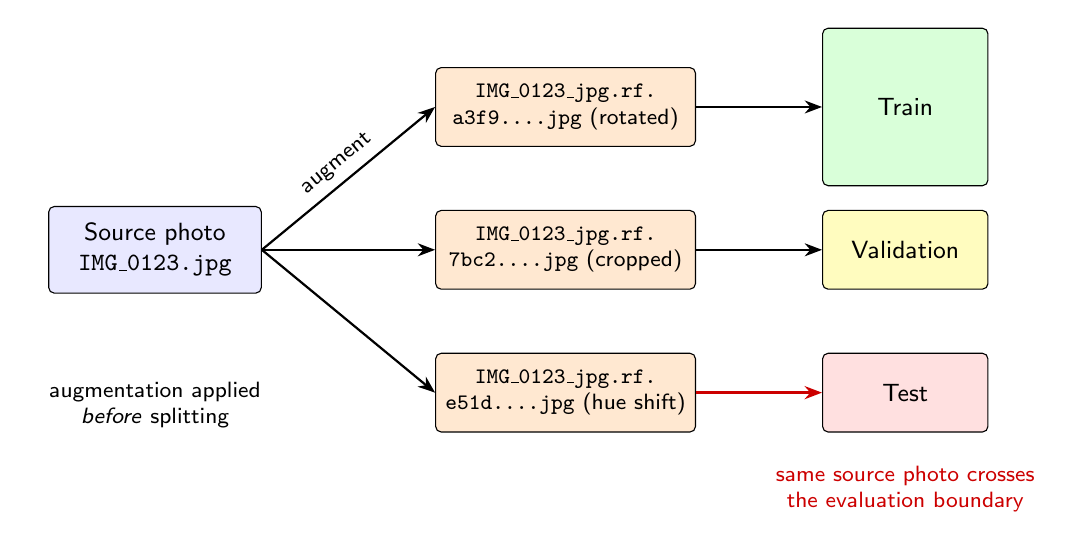
\begin{tikzpicture}[
  var/.style={draw, rounded corners=2pt, fill=orange!18, align=center, minimum width=33mm, minimum height=10mm, font=\footnotesize},
  split/.style={draw, rounded corners=2pt, align=center, minimum width=21mm, font=\small},
  arr/.style={-{Stealth[length=2.2mm]}, thick}]
\node[draw, rounded corners=2pt, fill=blue!9, align=center, minimum width=27mm, minimum height=11mm, font=\small] (src)
  {Source photo\\ \texttt{IMG\_0123.jpg}};
\node[var, right=22mm of src] (v2) {\texttt{IMG\_0123\_jpg.rf.}\\ \texttt{7bc2....jpg} (cropped)};
\node[var, above=8mm of v2] (v1) {\texttt{IMG\_0123\_jpg.rf.}\\ \texttt{a3f9....jpg} (rotated)};
\node[var, below=8mm of v2] (v3) {\texttt{IMG\_0123\_jpg.rf.}\\ \texttt{e51d....jpg} (hue shift)};
\node[split, fill=green!15, minimum height=20mm, right=16mm of v1] (tr) {Train};
\node[split, fill=yellow!25, minimum height=10mm, right=16mm of v2] (va) {Validation};
\node[split, fill=red!12, minimum height=10mm, right=16mm of v3] (te) {Test};
\draw[arr] (src.east) -- node[sloped, above, font=\footnotesize] {augment} (v1.west);
\draw[arr] (src.east) -- (v2.west);
\draw[arr] (src.east) -- (v3.west);
\draw[arr] (v1) -- (v1 -| tr.west);
\draw[arr] (v2) -- (va);
\draw[arr, red!80!black, very thick] (v3) -- (te);
\node[below=10mm of src, align=center, font=\footnotesize, text width=30mm] {augmentation applied\\ \emph{before} splitting};
\node[below=3mm of te, align=center, font=\footnotesize, text=red!80!black] {same source photo crosses\\ the evaluation boundary};
\end{tikzpicture}
\end{document}
